\documentclass[twocolumn,a4j]{jsarticle}
\bibliographystyle{junsrt}

\setlength{\topmargin}{-20.4cm}
\setlength{\oddsidemargin}{-10.4mm}
\setlength{\evensidemargin}{-10.4mm}
\setlength{\textwidth}{18cm}
\setlength{\textheight}{26cm}

\usepackage[top=15truemm,bottom=20truemm,left=20truemm,right=20truemm]{geometry}
\usepackage[latin1]{inputenc}
\usepackage{amsmath}
\usepackage{amsfonts}
\usepackage{amssymb}
\usepackage[dvipdfmx]{graphicx}
\usepackage[hang,small,bf]{caption}
\usepackage[subrefformat=parens]{subcaption}
\usepackage[dvipdfmx]{color}
\usepackage{listings}
\usepackage{listings,jvlisting}
\usepackage{geometry}
\usepackage{framed}
\usepackage{color}
\usepackage[dvipdfmx]{hyperref}
\usepackage{ascmac}
\usepackage{enumerate}
\usepackage{tabularx}
\usepackage{cancel}
\usepackage{scalefnt}
\usepackage{overcite}
\usepackage{otf}

\renewcommand{\figurename}{Fig.}
\renewcommand{\tablename}{Table }

\hypersetup{%
    hidelinks %リンクの色消し
}

\lstset{
basicstyle={\ttfamily},
identifierstyle={\small},
commentstyle={\smallitshape},
keywordstyle={\small\bfseries},
ndkeywordstyle={\small},
stringstyle={\small\ttfamily},
frame={tb},
breaklines=true,
columns=[l]{fullflexible},
xrightmargin=0zw,
xleftmargin=3zw,
numberstyle={\scriptsize},
stepnumber=1,
numbersep=1zw,
lineskip=-0.5ex
}

% キャプション後ろのダブルコロンを消す
\makeatletter
\long\def\@makecaption#1#2{%
  \vskip\abovecaptionskip
  \iftdir\sbox\@tempboxa{#1\hskip1zw#2}%
    \else\sbox\@tempboxa{#1 #2}%
  \fi
  \ifdim \wd\@tempboxa >\hsize
    \iftdir #1\hskip1zw#2\relax\par
      \else #1 #2\relax\par\fi
  \else
    \global \@minipagefalse
    \hbox to\hsize{\hfil\box\@tempboxa\hfil}%
  \fi
  \vskip\belowcaptionskip}
\makeatother


\makeatletter
\def\@maketitle
{
\begin{center}
{\LARGE \@title \par}
\end{center}
\begin{flushright}
{\large \@date}\\
{\large 京都工芸繊維大学 大学院 機械設計学専攻 計測システム工学研究室}\\
{\large M2 \@author}
\end{flushright}
\par\vskip 1.5em
}
\makeatother

\author{来代 勝胤 / KITADAI Masatsugu}
\title{令和5年度 4月度 共同研究 報告書}
\date{2023/04/25}

\begin{document}
\columnseprule=0.1mm
\maketitle

\section*{内容}
\begin{enumerate}[1.]
  \item 研究方針と研究計画
  \item 数値シミュレーション
  \item 研究発表について
  \item 5月の予定
\end{enumerate}

\section{研究方針と研究計画}
\begin{figure}[htbp]
  \footnotesize
  \begin{center}
    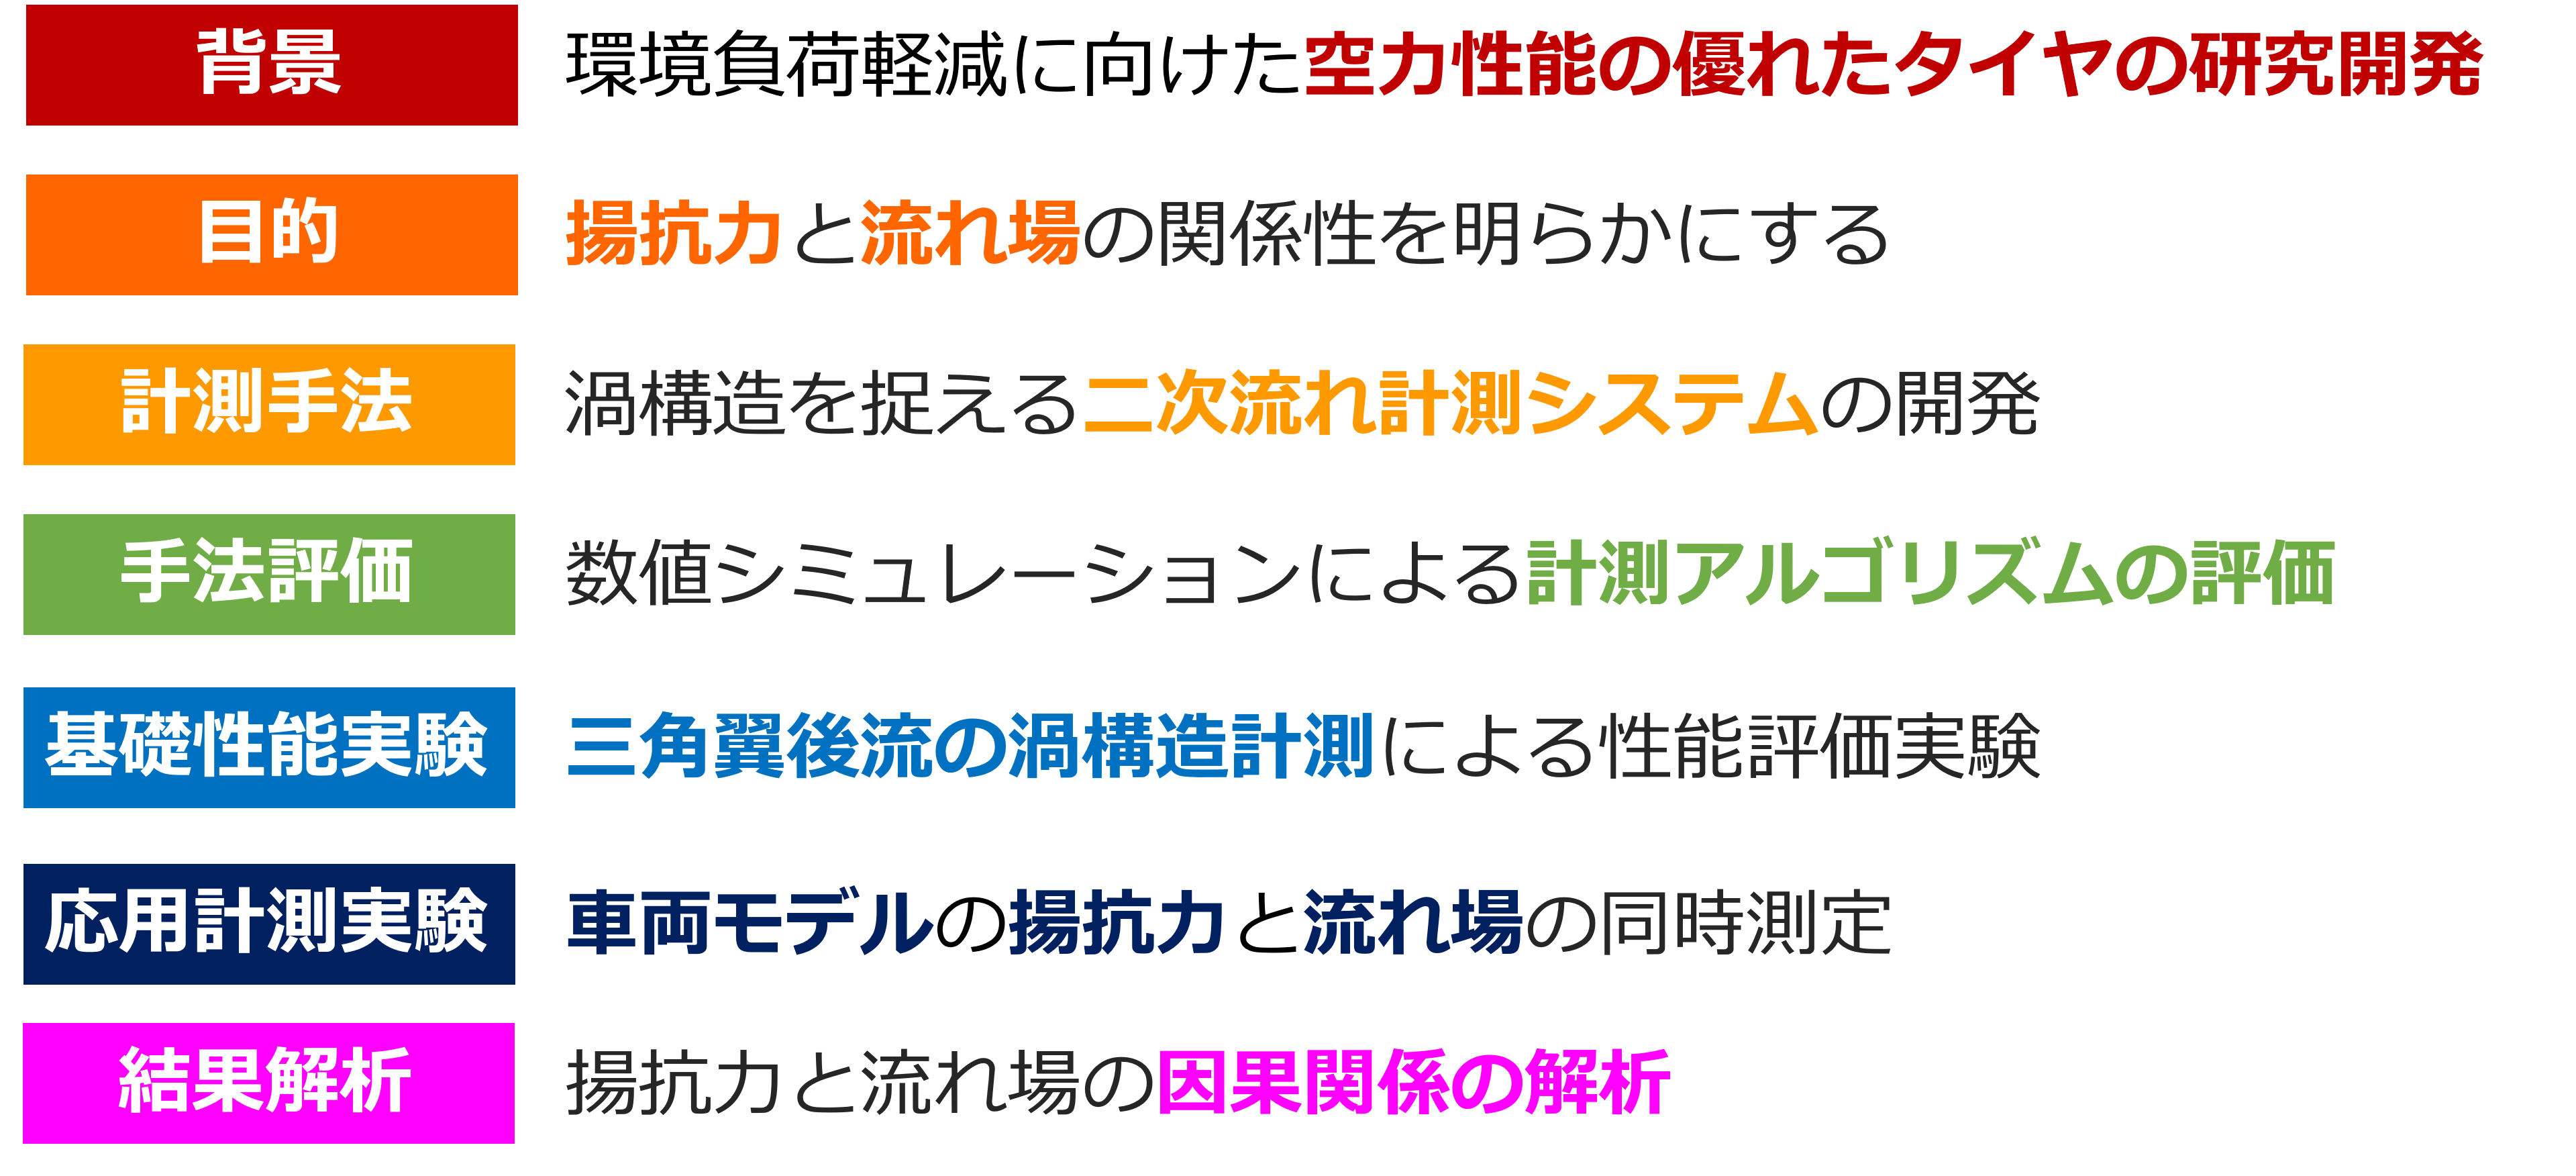
\includegraphics[width=85mm]{../images/schedule_2023.png}
  \end{center}
\end{figure}
2023年度は,以上の内容に沿って取り組む予定である.
これまで取り組んできた「二次流れの計測手法開発」を継続して行うと共に,
その定量的な性能評価および車両モデル周り流れの計測へと移行する.

\section{数値シミュレーション}
計測アルゴリズムの性能評価として,
数値シミュレーションを用いた誤差評価を行う.
今回は,3次元の定常解が示された流れ場を用いて
実験条件を再現する.今月は数値シミュレーションの詳細について報告する.\\

\subsection{再現する回転壁付近の流れ場}
\begin{figure}[htbp]
  \footnotesize
  \begin{center}
    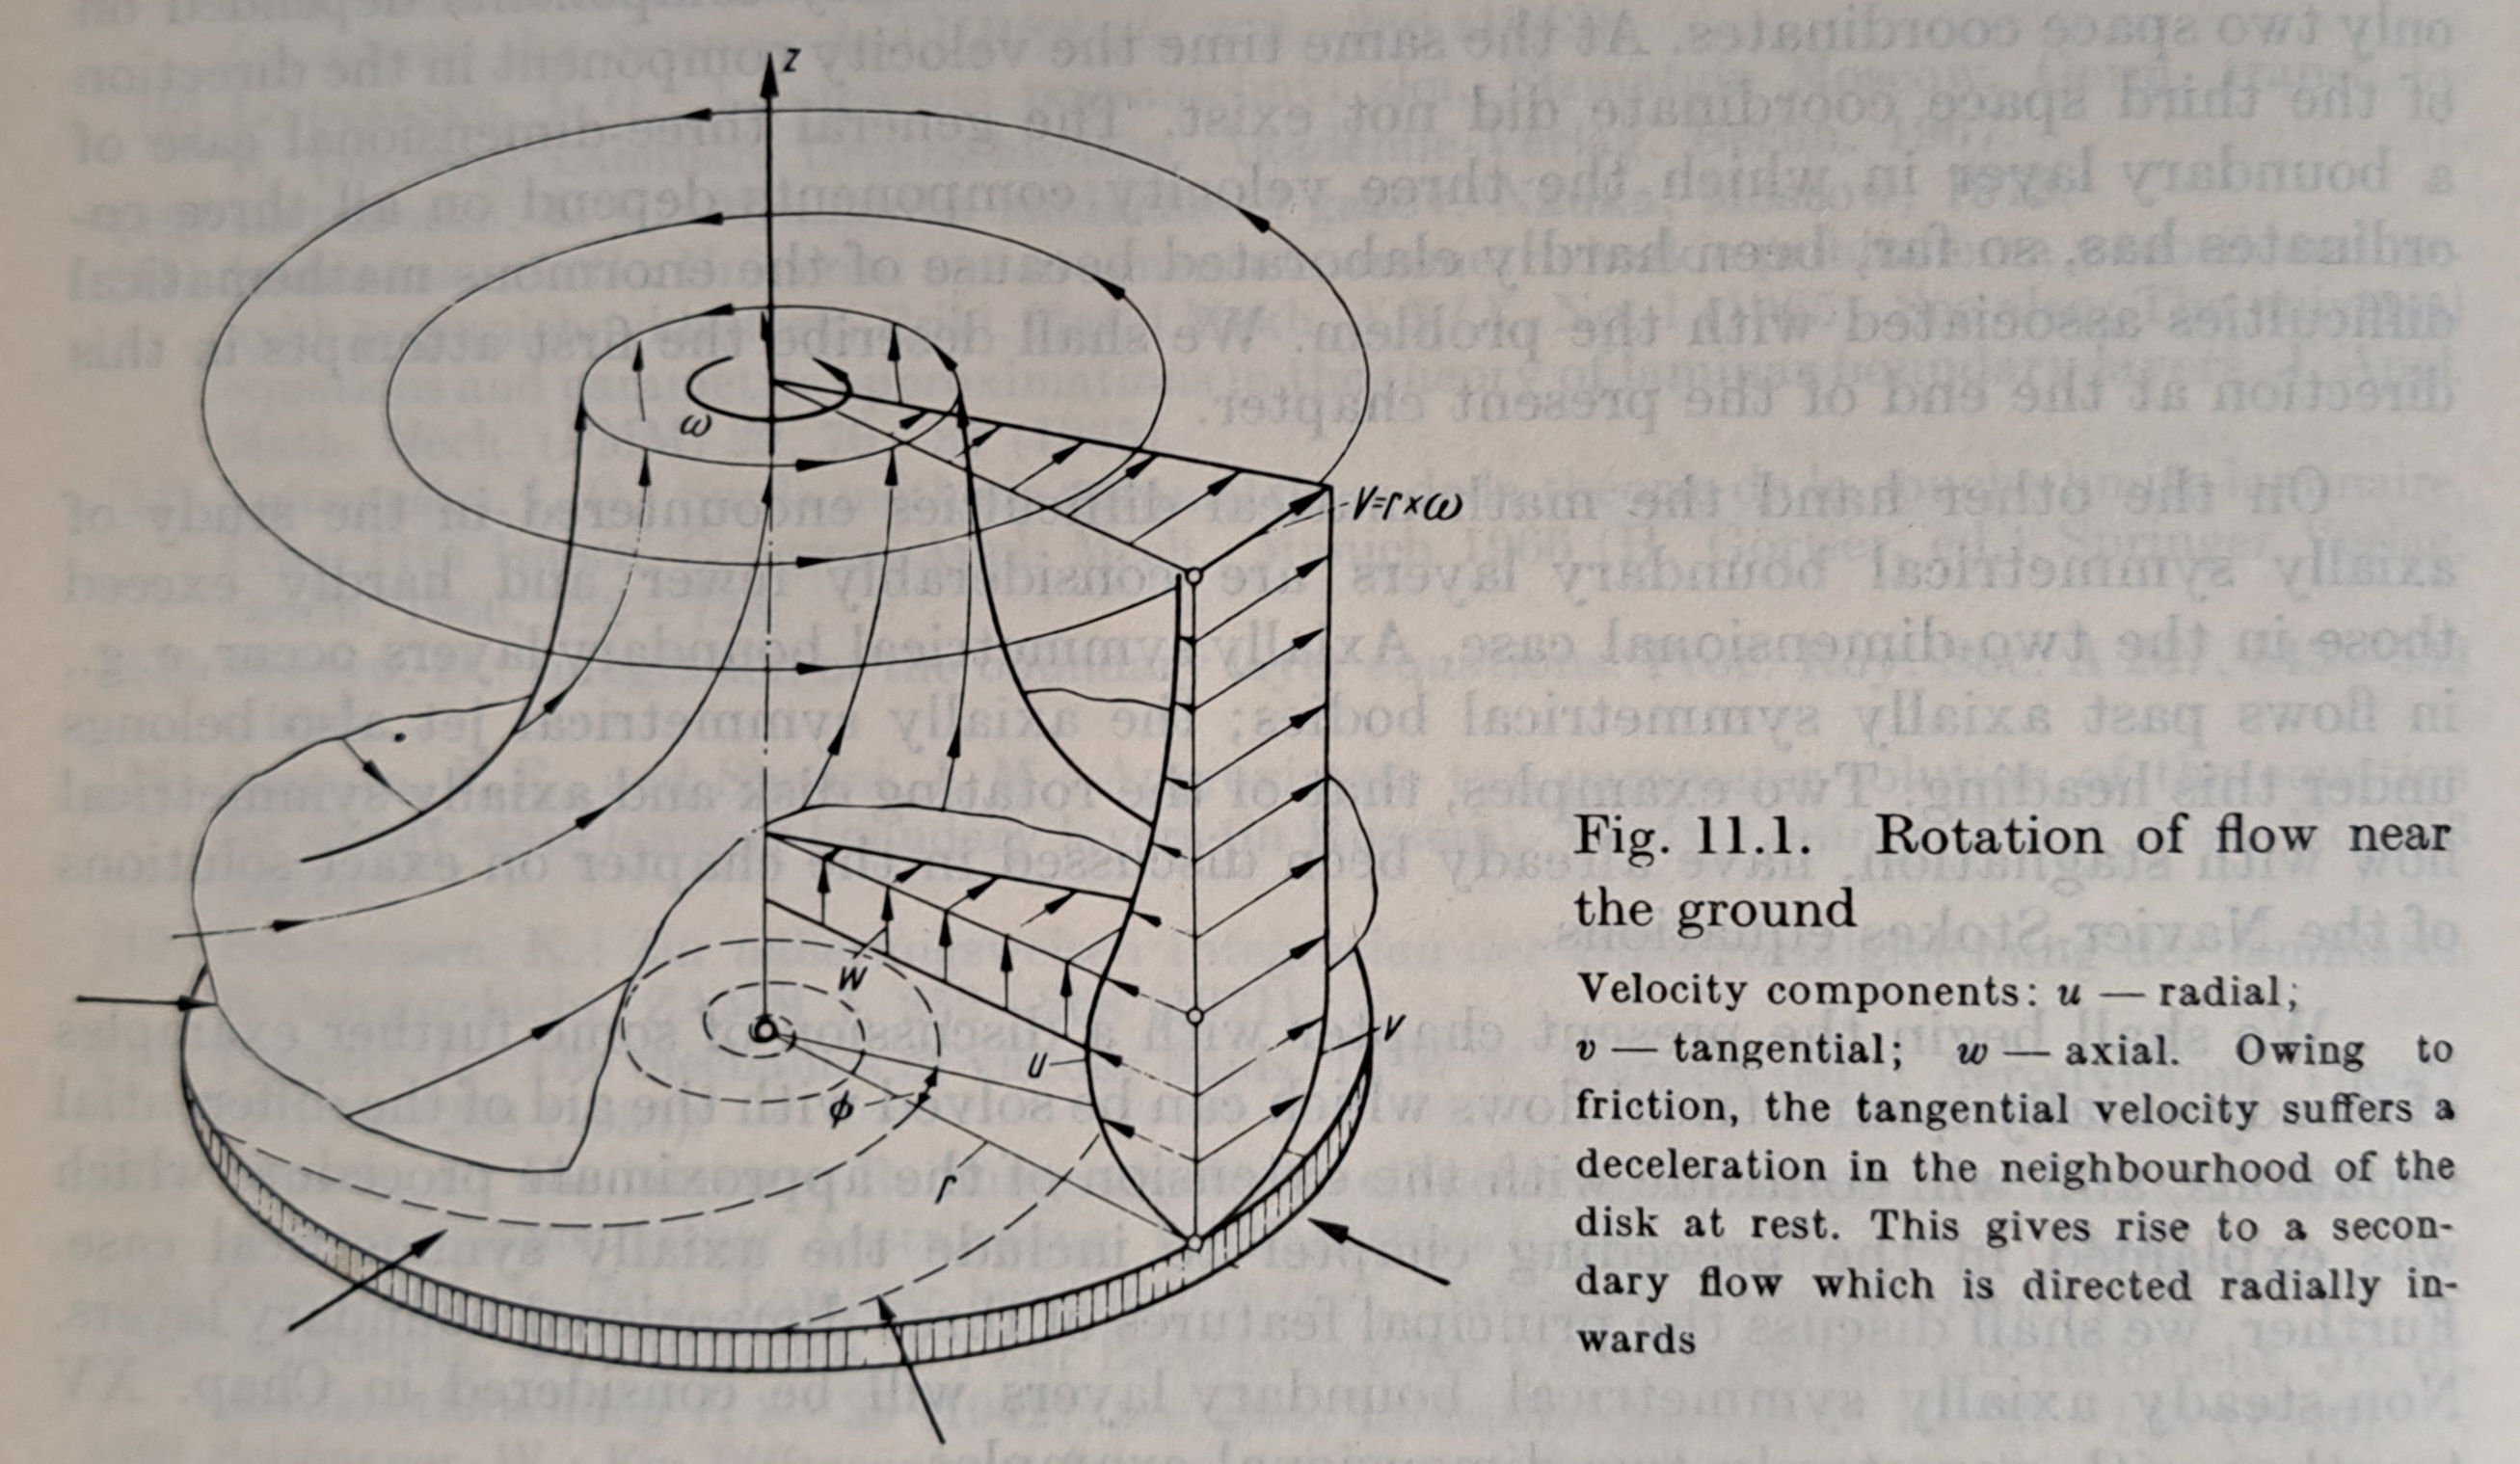
\includegraphics[width=75mm]{../images/Boundary-Layer_Theory_Fig.11.1.jpg}
    \caption{Rotation of flow near the ground}
  \end{center}
\end{figure}

\newpage

\subsection*{【流れの解析解】}
\begin{eqnarray*}
  \zeta &=& z \sqrt{\frac{\omega}{\nu}}\\
  \\
  V_r &=& r \omega F \left(\zeta\right)\\
  V_\theta &=& r \omega G \left(\zeta\right)\\
  u &=& \sqrt{\nu \omega} H \left(\zeta\right)
\end{eqnarray*}

\subsection*{【境界条件】}
\begin{table}[hbtp]
  \centering
  \begin{tabular}{ c c c c }
    $x=0$      & $V_r=0$ & $V_\theta =0$        & $u=0$ \\
    $x=\infty$ & $V_r=0$ & $V_\theta =r \omega$ &       \\
  \end{tabular}
\end{table}

\begin{figure}[htbp]
  \footnotesize
  \begin{center}
    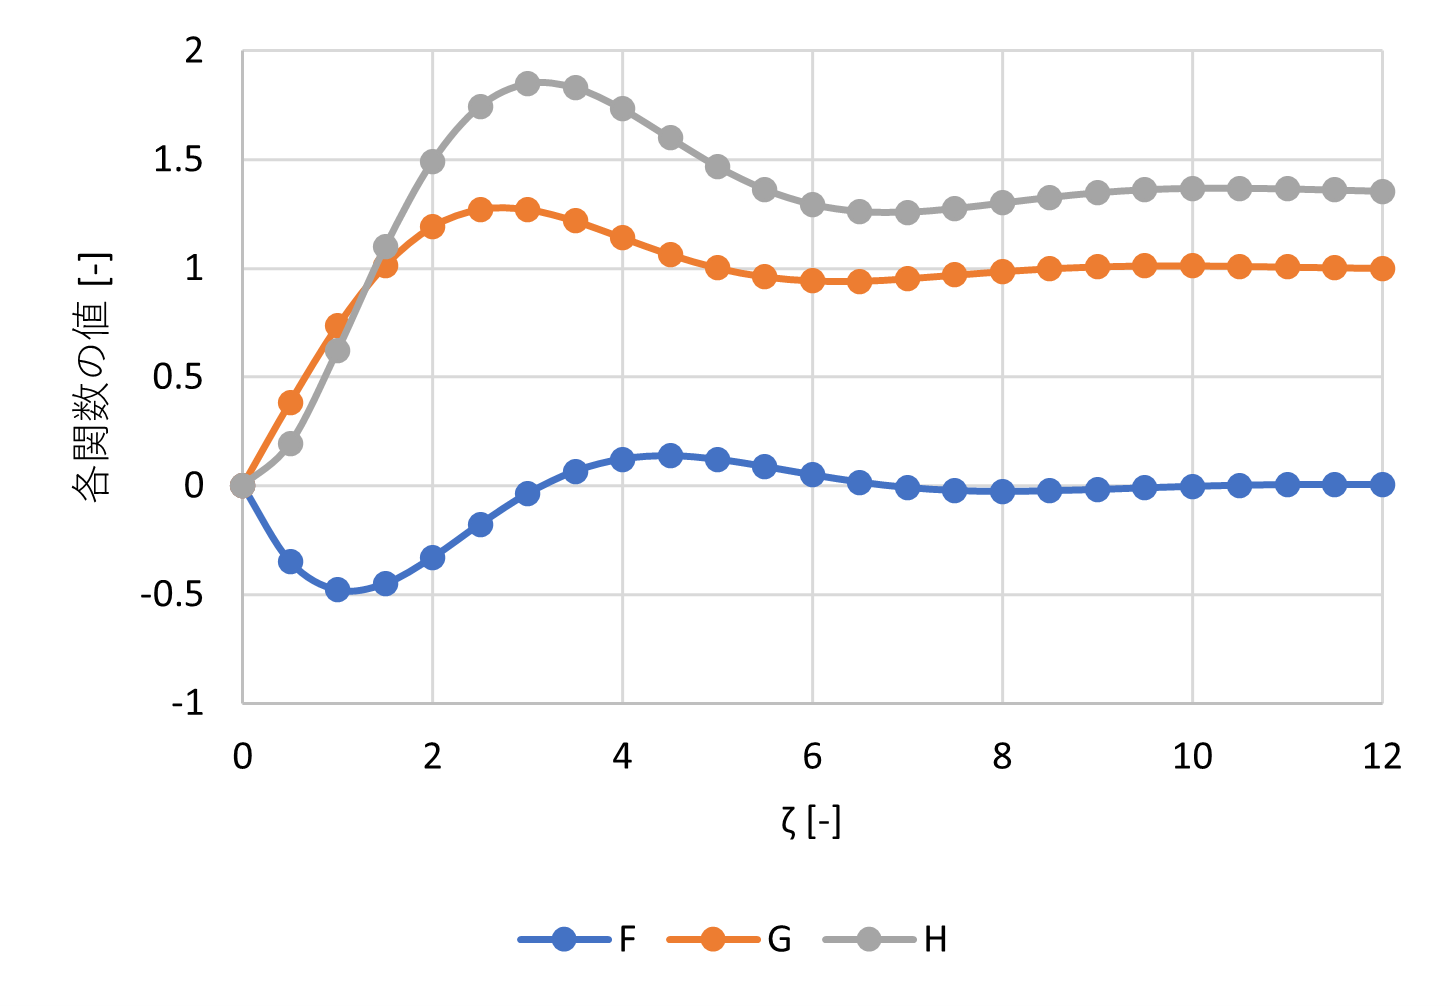
\includegraphics[width=75mm]{../images/function_graph.png}
    \caption{各関数の推移}
    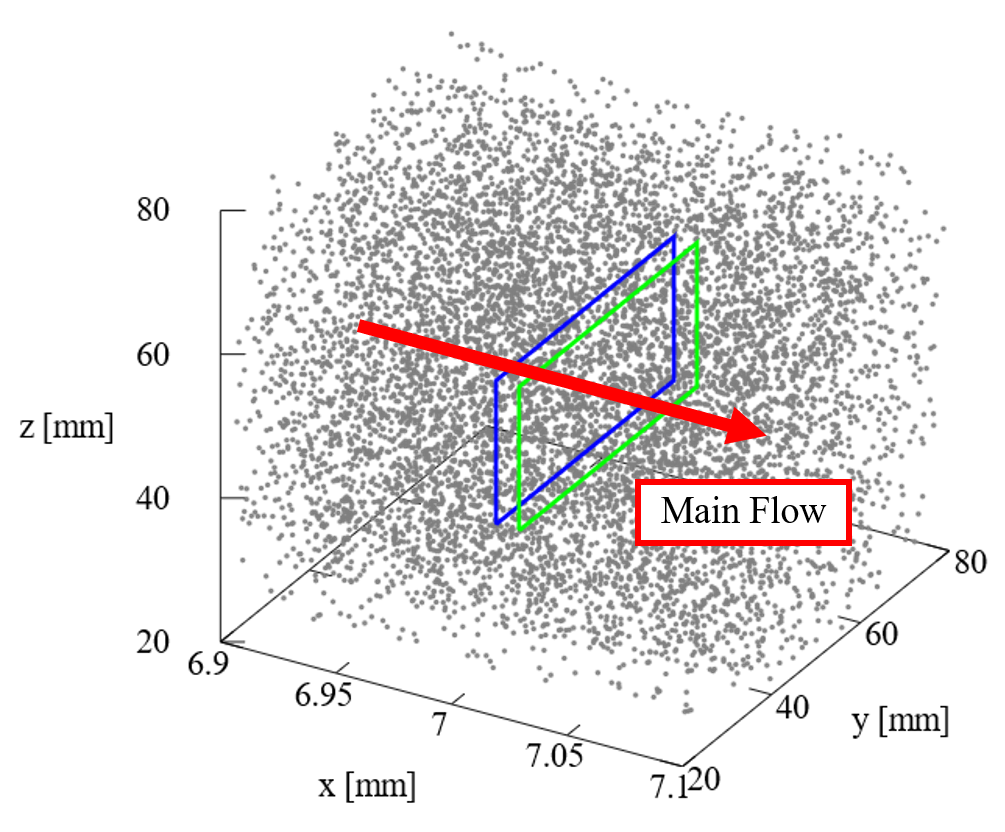
\includegraphics[width=85mm]{../images/Numerical_simulation_of_flow.png}
    \caption{数値シミュレーションの概略図}
  \end{center}
\end{figure}

\newpage
\subsection{数値シミュレーションの条件}
数値シミュレーションは,回流水槽の実験条件と対応させて設定している.

\begin{table}[hbtp]
  \label{table:data_type}
  \caption{シミュレーション条件}
  \centering
  \begin{tabular}{ c c | r l}
    \hline
    粒子数密度              & $n$          & 140                    & [個/枚]            \\ \hline
    壁の回転速度            & $\omega$     & 10                     & [deg/s]            \\ \hline
    動粘性係数              & $\nu$        & $1.004 \times 10^{-6}$ & [$\mathrm{m}^2$/s] \\ \hline
    $\mathrm{LLS}_1$ の位置 & $x_0$        & 7.000                  & [mm]               \\ \hline
    $\mathrm{LLS}_1$ の厚み & $T_1$        & $3.086\times 10^{-3}$  & [mm]               \\ \hline
    $\mathrm{LLS}_2$ の厚み & $T_2$        & $9.259\times 10^{-3}$  & [mm/s]             \\ \hline
    LLS 間の距離            & $\Delta x$   & $9.645\times 10^{-3}$  & [mm/s]             \\ \hline
    撮影範囲                & $y \times z$ & $40 \times 20$         & [mm]               \\ \hline
    画像サイズ              & $w \times h$ & $800 \times 400$       & [px]               \\ \hline
  \end{tabular}\\
  \vskip\baselineskip
  \caption{実験条件(参考)}
  \begin{tabular}{ c c | r l}
    \hline
    粒子数密度              & $n$            & 70                     & [個/枚]            \\ \hline
    流れの回転速度          & $\omega'$      & -                      & [deg/s]            \\ \hline
    動粘性係数              & $\nu'$         & $1.004 \times 10^{-6}$ & [$\mathrm{m}^2$/s] \\ \hline
    $\mathrm{LLS}_1$ の位置 & $x'_0$         & -                      & [mm]               \\ \hline
    $\mathrm{LLS}_1$ の厚み & $T'_1$         & 1.000                  & [mm]               \\ \hline
    $\mathrm{LLS}_2$ の厚み & $T'_2$         & 3.000                  & [mm/s]             \\ \hline
    LLS 間の距離            & $\Delta x'$    & 3.125                  & [mm/s]             \\ \hline
    撮影範囲                & $y' \times z'$ & $100 \times 50$        & [mm]               \\ \hline
    画像サイズ              & $w' \times h'$ & $800 \times 400$       & [px]               \\ \hline
  \end{tabular}
\end{table}

\subsection{数値シミュレーションの解析}
作成した数値シミュレーションについて,
現在の計測アルゴリズムを適用した結果を以下のFig.4 に示す.
今後は,真値との比較を行い定量的な誤差評価を行う.
\begin{figure}[htbp]
  \footnotesize
  \begin{center}
    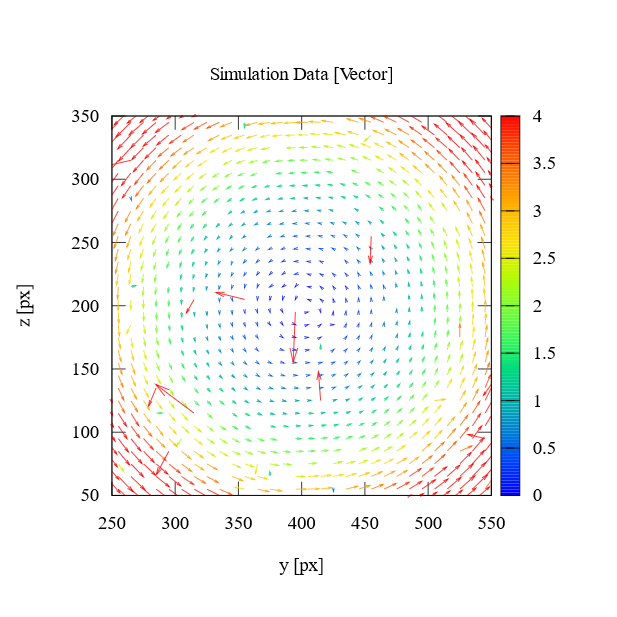
\includegraphics[width=73mm]{../images/simulation_result.png}
    \caption{数値シミュレーションによる流れ場の解析結果}
  \end{center}
\end{figure}

\newpage
\section{研究発表について}
以下の項目について,研究発表を予定している.
\begin{enumerate}[(1)]
  \item 実験結果:実験による計測結果について
  \item 実験手法:計測手法と画像校正法について
  \item 性能評価:計測アルゴリズムの性能評価について
\end{enumerate}

\subsection{第51回 可視化情報シンポジウム}
\begin{table}[hbtp]
  \label{table:data_type}
  \begin{tabular*}{9.5cm}{ c | c }
    \hline
    \textgt{題目} & \begin{tabular}{c} 多重カラーLLSを用いた供試体を過ぎる\\二次流れのPIV計測  \end{tabular}        \\ \hline
    \textgt{内容} & \begin{tabular}{c} 三角翼後流及び車両モデル周りの流れ場\\の計測結果について  \end{tabular}        \\ \hline
    \textgt{日時} & 2023/8/8 - 8/9                   \\ \hline
    \textgt{会場} & 北海道 小樽市 グランドパーク小樽 \\ \hline
    \textgt{登録締切} & 2023/4/19                        \\ \hline
    \textgt{原稿締切} & 2023/5/31                        \\ \hline
  \end{tabular*}
\end{table}

\subsection{日本実験力学会 2023年度年次講演会}
\begin{table}[hbtp]
  \label{table:data_type}
  \begin{tabular*}{9.5cm}{ c | c }
    \hline
    \textgt{題目} & 未定                             \\ \hline
    \textgt{内容} & \begin{tabular}{c} 回流水槽を用いた二次流れの計測方法および\\画像の校正方法について  \end{tabular}        \\ \hline
    \textgt{日時} & 2023/8/29 - 8/31                 \\ \hline
    \textgt{会場} & 和歌山県 和歌山市 和歌山城ホール \\ \hline
    \textgt{登録締切} & 2023/5/15                        \\ \hline
    \textgt{原稿締切} & 2023/6/30                        \\ \hline
  \end{tabular*}
\end{table}

\subsection{ISTP-33}
\begin{table}[hbtp]
  \label{table:data_type}
  \begin{tabular*}{9.5cm}{ c | c }
    \hline
    \textgt{題目} & \begin{tabular}{c} Performance Evaluation of PIV Measurement \\ of Secondary Flow using Multi-Color LLS \end{tabular}        \\ \hline
    \textgt{内容} & \begin{tabular}{c} 数値シミュレーションを用いた\\計測手法の精度評価の結果について \end{tabular}        \\ \hline
    \textgt{日時} & 2023/9/24 - 9/27                 \\ \hline
    \textgt{会場} & 熊本県 熊本市中央区 熊本城ホール\\ \hline
    \textgt{登録締切} & 2023/4/30                        \\ \hline
    \textgt{原稿締切} & 2023/5/31                        \\ \hline
  \end{tabular*}
\end{table}

\section{5月の予定}
\begin{itemize}
  \item 数値シミュレーションを用いた誤差評価
  \item 三角翼後流の流れ場計測
  \item 車両モデル周りの流れ場計測
  \item ISTP 論文提出 (5/30)
  \item 可視化情報シンポジウム 原稿提出 (5/30)
\end{itemize}


\end{document}